\documentclass[11pt,a4paper]{report}

\usepackage[utf8]{inputenc}
\usepackage{amsmath}
\usepackage{natbib}
\usepackage{url}
\usepackage{listings}
\usepackage{graphicx, wrapfig}
\usepackage[font=small,labelfont=bf]{caption}
\usepackage{float}
\usepackage{afterpage}
\usepackage{appendix}
\usepackage{minted}
%Fancy Header-----
\usepackage{fancyhdr}
\setlength{\headheight}{14pt}%
\pagestyle{fancy}
\fancyfoot{}
\renewcommand{\footrulewidth}{0.0pt}
\renewcommand{\headrulewidth}{0.0pt}
\lhead{CMP3060M - Project - 
Assessment Item 2 - Project Report}
\rhead{}
\fancyfoot[R]{\thepage}
\fancyfoot[L]{PRO14514822 - Owen Prosser}
\fancypagestyle{plain}{\pagestyle{fancy}}
%-------------
%Fancy Header-----
\usepackage{afterpage}
\newcommand\blankpage{%
    \null
    \thispagestyle{empty}%
    \addtocounter{page}{-1}%
    \newpage}
\graphicspath{ {images/} }
%-------------

%Harvard Referencing
\bibliographystyle{agsm}

%Setup the title
\title{
	{AN INVESTIGATION INTO THE DEVELOPMENT AND EFFECTIVNESS OF COMPUTER-VISON FALL DETECTION SYSTEMS AT THE UNIVERSITY OF LINCOLN}\\
	{\large University Of Lincoln}
}
\author{PRO14514822 - Owen Prosser}
\begin{document}
%Insert the title
\maketitle

\begin{abstract}
\emph{The overall aim of this project is to create a Fall Detection System using the Python programming language and its OpenCV library. This system is intended for to assist families, or care-providing professionals, who are responsible for the well-being of the elderly but cannot for whatever reason monitor them at all times. It is designed to alert any kind of care-giver in the event that an elderly person has had a fall and potentially hurt themselves potentially requiring medical attention, or just some reassurance and compassion.}
\end{abstract}

%\afterpage{\blankpage}

\tableofcontents

%\afterpage{\blankpage}

\chapter{Literature Review}
\section{Background}
According to the World Health Organisation a fall is the second leading cause of "unintentional injury deaths" worldwide, making this an issue of the highest severity \citep{Cruz_Fall_detection_wearable_device}. The population is aging in most western countries. In the US, in the 28 years from 1980 from 2008, the share of the population over 60 has nearly doubled from 9.9 million to 18.6 million \citep{Siracuse_Health_care_and_socioeconomic}\% of both independent and institutionalised persons over the age of 75 are estimated to experience a traumatic fall in a year \citep{Sixsmith_A_smart_sensor_to_detect}, putting the elderly at a significantly higher risk of "injury to the head, neck, and pelvis than younger individuals"  These falls a huge issue for the elderly population as it is estimated that 90\% of geriatric injuries are caused by falls \citep{boltz_Injuries_and_outcomes}. This puts a huge strain on hospitals as well as families who care for elderly relatives. A system for detecting these falls should they occur could assist carers for the elderly as they would not have to be with the cared at all times. This would both reduce the workload for the carer and give back some privacy and independence. It has also been shown that "longer the lie on the floor, the poorer is the outcome of the medical intervention"\citep{Li_A_microphone_array}. A detection system which could alert a care giver quickly could reduce the delay between the fall and provision of medical assistance increasing the chances of a good recovery and lowering distress for the patient.

\section{Available Systems}
There are many currently available alarm systems for detecting human falls. These are generally split into two categories; user-activated systems where the user manually actives an alarm after a fall, and automatic systems where the alarm is triggered without user interaction once a fall is detected \citep{Alwan_A_smart_and_passive_floor-vibration}. 

\section{Wearable Systems}
A large portion of these automatic systems require the user to wear specialised equipment or carry a device with them at all times. These devices are then used to motion and/or location of the user. One of these systems uses the accelerometer built into most modern smart phones to detect falls \citep{Tsinganos_A_smartphone-based_fall}. This works by sensing a sudden change in acceleration of the device. This system is fairly accurate with a precision of 91.8\% but has a few fundamental drawbacks. Firstly, the system's accuracy is affected by how the user is carrying the phone their body and of course it has a 0\% accuracy when the phone is not being carried or is not running the app. Many systems attack specialised hardware to the body of the user to measure their acceleration to detect falls. One of these systems uses a 'pendant' worn around the user's neck \citep{Santiago_Fall_detection_system}. The detection systems work in a similar way to the previous smartphone-app-bases system, this time with the pendant having dedicated hardware to measure changes in acceleration rather than using the multipurpose sensors built into a smartphone. This pendant then communicates with a smartphone app to trigger an alert if a fall is detected. This system has a very similar accuracy rate of 92\% but has the advantage that this should be very consistent as the detector will always be placed in the same area of the user's body compared to a smartphone. Another system uses a unit of sensors attached to the belt of the user \citep{Cruz_Fall_detection_wearable_device}. Whilst the accuracy of the system is not present in this paper it could be assumed that it would be similar to that of the previous system as they both feature a similar hardware implementation and methodology for establishing the acceleration threshold for determining a fall. Without evidence of a significant improvement in the quality of detection this system appears less practical than the previous system as the belted sensor array is bulkier and probably less comfortable to wear making them an "unfavourable choice for the elderly" \citep{fallDetectionInvestigation}. These systems, however, still requires that the user wear a specialised piece of hardware at all times for the system to be functioning although this is better than having to carry a smartphone at all times. One severe limitation of all of the smartphone-based systems is that they require the user to already own a smartphone. This is a limiting factor because whilst smartphone adoption is on the rise among the over 55 age group only 30\% of this category currently own a smartphone \citep{Berenguer_Are_Smartphones_Ubiquitous}. The potential user base for a fall detection system could be greatly expanded if the system was functional on its own without being reliant on the user's smartphone connection to the Internet to trigger and alarm in the event of a fall. As many elderly people "are having difficulties in using modern smart devices" \citep{William_Cognitive_modeling_in_human_computer_interaction} a system which does not require the direct interaction of the user to function could be more effective at detecting falls as it can be passively running in the background in no way reliant on input from the user or their aptitude for technology.

\section{Passive Systems}
Passive systems use a variety of sensing methods to the detect falls, including cameras, Infra-Red (IR) thermal-imaging cameras or ultra-sonic sensors. One of the most effective of these systems uses ultrasonic sensors to detect the area of the floor of a room which is covered by the user. When walking around the house normally the user's feet will only cover a small section of the floor space, in the event of a fall the user's body will cover a larger area of the floor, the system will detect this as a fall \citep{Chang_Human_fall_detection_based_on_event}. This system is very accurate with "up to 98\% precision" but does require a large amount of hardware to be installed around the perimeter of each room where fall detection is required. Another passive system uses a ceiling-mounted IR camera to gather a top down heat map of the room. \citep{Hayashida_The_use_of_thermal_ir_array}. When the user is moving around the monitored space normally the camera will perceive a small area being at a higher temperature than the rest of the room. If the user is to fall over in view of the thermal-camera their thermal signature will appear larger to camera allowing it to detect a fall. This system is effective at its goal of detecting falls with a "robust fall recognition rate (over 94\%)" but requite specialised thermal imaging hardware. This hardware, at its current cost, would be prohibitively expensive not only to this project but also to the system's end user. One other passive system utilises a circular array of 8 omni-directional microphones to detect a fall based on the noise of contact with the floor \citep{Li_A_microphone_array}. The main drawback of this type of system is that its accuracy is somewhat dependent on the acoustic conditions of the room. Any background noise from traffic or a television can mask the sound of a fall potentially allowing for it to be missed. This is not shared by systems which rely of camera (including thermal imaging cameras) as these are not affected by interference.

\section{Detecting Falls}
The Passive Fall-Detection systems detect when the user has fallen in a number of different ways. One system uses the angle of the Major and Minor axes of an "approximate ellipse" around the silhouette of the user \citep{rougier2007fall}. This is shown to work effectively as the referenced system was tested with 17 falls and correctly detected 15 of them \citep{rougier2007fall}. This solution is also relatively understandable and could potentially contribute to a straight-forward implementation as it requires no additional or specialised hardware. Some of the other passive systems require hardware other than a standard web cam to operate. For example one passive system uses the RGB-D (Red, Green, Blue and Depth) built into the Microsoft Kinect depth sensor \citep{kinectPassiveDetection}. Another visual camera-based system uses ceiling-mounted overhead cameras cameras \citep{nait2004activity}. This detection method work by "shape change analysis as well as inactivity detection" from an overhead view \citep{fallDetectionInvestigation}.

\section{Conclusions}
Many elements of the discussed research is relevant and will have an effect on this project. Firstly it is important that the system is active at all times as a fall can be severely damage the health and wellbeing of an elderly person. Consequently the Fall Detection System should not be configured or operated by the monitored person as they are likely to be old and thus not technologically adept. The user would also benefit from any specialised wearable-hardware being a requirement for the operation of the system. This would allow the user a fuller freedom of movement and more comfort in their home.
This Passive system will also function using a method similar to that of \cite{rougier2007fall}. This is due to certain limitations of this project. In this project it is not feasible to acquire and use non-standard hardware as mention in Section 1.5 for reasons of both cost, and the time restrictions placed on the project. As it would take significant effort to configure and develop such a system.

\chapter{Methodology}

\section{Project Management}
This project was developed using an agile methodology. The development of the artefact was divided into many one week long sprints each beginning/concluding with a meeting with the project supervisor. Each of these meetings began with a brief discussion of the progress made during the previous week. This part of the meeting was then followed by a discussion of the tasks to be undertaken before the next meeting. This follows the structure of an iterative methodology.

An iterative methodology also focuses on breaking down the entire project into small parts, each of these parts in then set to be completed during one of the many sprints. At the beginning of the development process the requirements of the project are analysed to find how they can be best be divided into their component parts for each of the sprints. The most important factor during this part of the process is to have a well-defined set of requirements. This allows for the project to be accurately broken down without having to repeat this process again when the requirements become more clearly defined. This was useful during this project as the require were very well-defined at the beginning of the project and have not changed during the development. The progress of the project is made easier to track when it is divided into many parts in this way. Throughout the entire project it is known how many parts are left to complete and what is required to complete each of them. The progress can also be precisely known because the project is being undertaken by an individual rather than a team. This means that it is not required to understand how other members of the team are working what progress they are making.

Another of the main purposes of using an iterative methodology is to allow the individual to be more adaptable if, and when, an obstacle to development does arise \citep{Wiley_Project_Management}. After a break in productivity due to a change in the system's requirements or other unforeseen circumstance, an iterative project management methodology can adapt to this change. This is due to the structure of having many regular meetings, each with its own set of goals. These meetings allow for a team or individual developer to realign and reorder the upcoming tasks based on the best way to navigate this landscape of new requirements. One example of this used during the completion of this artefact; there were many other unrelated tasks which needed to be completed in parallel with this project. This caused some delays throughout the development as these other tasks could often have their own delays and unforeseen changes. This kind of individual sprint is only possible with a small scale development such as this, usually an individual would not be able to focus themselves in one particular area for an extended period of time without it being detrimental to their other responsibilities if they were trying to run a small one-person business for example. However, this approach can have some drawbacks in terms of a project such as this. As this is a small project undertaken by an individual without much oversight, there is the possibility of getting lost and not making sufficient progress towards the overall goal caused by constantly changing direction with each sprint.

An iterative Agile methodology is advantageous over an non-agile methodology like Waterfall. When using Waterfall, for example, each stage of development has to be completed before the next can begin. This can cause large delays when one part of the project is experiencing delays. This would be particularly problematic for a project such as this as delays can be common for all parts of the development for many reasons. Firstly, many other unrelated tasks were also required their own dedicated time to complete during the development of the artefact. This would have caused long delays under a Waterfall development method as it would have prevented development on any other part of the artefact until these other tasks had been fully completed. Also as some time was required to be spent researching and learning how to use some of the vital components of this project, this would have caused other parts of the development to completely stall under the older, non-agile Waterfall methodology. 

\pagebreak

\section{Software Development}
When creating any piece of software in any confined timescale it is important that there is some system for creating the software in an efficient manner. In order to do this effectively it has be managed within the limitations of the project at hand. This project has many factors which impact the available software engineering methodologies could be effectively employed to increase the speed of development and improve the quality of the artefact in relation to its original aim and objectives. The main factors which affected how this development of the project was carried out were that, firstly, this was a project for one individual to complete, it had a very strict deadline for completion which could not be extended, there were many other unrelated tasks which need to be completed in parallel, and also there were many unfamiliar components to be used for the development of the system which needed specific time set aside to be researched and learned how to be used. This project did however have one quality to the benefit of various Software Engineering Methodologies; the project had very well defined requirements from the beginning which can be vital during the planning stages which are an important part of many methodologies.

The oldest, and still one of the most commonly used development methodologies, is the Waterfall method \citep{shaydulin2017agile}. This methodology was not used for a number of reasons. Firstly, as the time to complete this project was limited the Waterfall methodology could have contributed incorrectly allocating time to certain areas of the project where it was not as needed as in others. This would have been due to the strictly linear structured nature of the methodology dictating that some parts of the project (such as requirement gathering and analysis) had to be completed before other stages could begin \citep{shaydulin2017agile}. This would have been an issue for this project as it carried out by an individual with other concerns during the development. Without being able to switch between different tasks and areas of the project as the available time permitted within a busy schedule the development could have stagnated. The Waterfall methodology has a rigid structure which does not allow the developer(s) to repeat a stage without completing all subsequent stages until the end of the cycle \citep{WaterfallPresentation} this would not allow for the software to be tested during the development as this would have to added as an additional stage at the end of the Waterfall cycle. This would have been detrimental to the development of the artefact because it relied on testing throughout the development to ensure that it was functioning correctly and any new features that had been added since the last set of tests had not introduced any new bugs.

One common methodology that could be applied to the project is Extreme-Programming (XP). Elements of this methodology were used during the development of the artefact. This was because "XP keeps short development cycles with incremental design and planning" \citep{XPsharma2016analysis} allowing the artefact to developed in small sections which could be individually designed and tested. XP "follows a ... testing strategy and restricts the propagation of the risk in the later stages" \citep{XPsharma2016analysis}. This allowed the addition of features to carry little risk of delay. If this had been done using a Waterfall methodology the software would have to be mostly completed before any tests could be carried out, increasing the time needed to resolve any issues that may be found as there would have been a larger code base to work on. This is described by \cite{XPsharma2016analysis} as the Waterfall or other non-agile methodology "tend to develop a faulty system". In addition to this XP has the flexibility to "accommodate the implementation of functionality" \citep{XPsharma2016analysis} which was useful as the artefact was developed in stages adding one feature at a time which was then tested. The increase in development speed is shown in figure \ref{fig:XPvsWater}. However not all aspects of XP were used, as there are multiple which did not apply to the specific aspects of this project. For example "XP is a software methodology that focuses on the pair programming" and "encourages a high degree of interactions between team members" \citep{XPsharma2016analysis} which of course could not be used as this was a project entirely completed by one individual. Also Extreme Programming "adapts [to] the changes in the project"

\begin{figure}
 \centering
 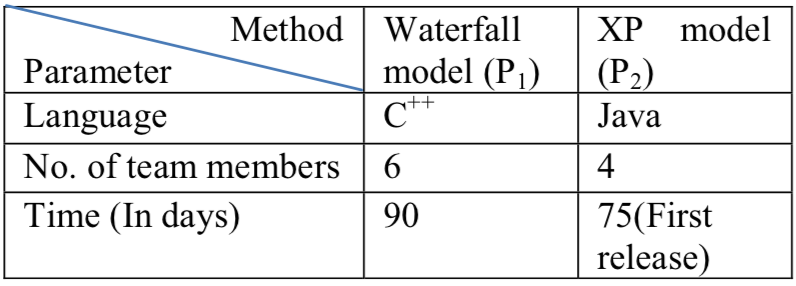
\includegraphics[scale = 0.45]{XP_vs_Waterfall.png}
 \caption{Table showing a comparison in development time for both Waterfall and XP 		methodologies \citep{XPsharma2016analysis}.}
 \label{fig:XPvsWater}
\end{figure}

As the development of the project was undertaken by an individual with a limited amount of available time as other tasks also required their own time and attention through the development process of this project the Kanban methodology was useful. One of the main features of the Kanban methodology is limiting the current workload on the team, or in this case the individual \citep{Kanban_lei2017statistical}. In this methodology only two parts of the project can be in active development at once. To start development one another part one of the in-progress tasks has to be completed. This helped to limit the current scope of the development to save time and prevent a lack of focus when balancing with other unrelated tasks.

This project had many limiting factors which dictated which parts of the development could be optimised with Software Engineering Methodologies it was important that the appropriate development system was used to deliver a working artefact on time. To do this it was not possible to use all aspects of one methodology to develop the artefact, parts had to be taken from multiple methodologies. For example the focus on smaller segments of the project by limiting the amount of items of work in progress from Kanban and the fast-paced test-focused style from Extreme Programming.

\section{Tool-Sets and Machine Environments}

The tools used in any project are very important to the finished artefact. This section will document the tools used as well as how, and why, they were chosen for their respective roles in the project.

Arguably the most important tool used for the creation of the project is the programming language itself. In the case of this project, the language used was Python \citep{Python}. This language was used for many reasons. Firstly, it is compatible with many languages which are useful to the project. This includes the OpenCV library which is vital to the project \citep{OpenCV}. Python was also used because it is able to be run on many different platforms including Mac OS, Windows and Linux systems. This is important to this artifact because the final implementation is intended to be run on a small system such as a Raspberry Pi so that it can be placed in a room and run permanently. It also a fast language to write, not requiring as many lines of code to accomplish a task as would be required in a language such as C++. This allows for faster development which can be more effectively partnered with an agile Software Engineering Methodology.    

The OpenCV library is used in some way for all components of the artefact which deal with video or image files. This library was chosen as it is the industry standard for computer vision libraries "companies like Google, Yahoo, Microsoft, Intel..." \citep{OpenCV}. Without the use of this library the project would be almost impossible to complete, especially within the timescale for this project to be completed. The scope of the project would increase by many orders of magnitude if all of the libraries' functions were rewritten for this project. Using OpenCV for this purpose also has another benefit, the library is written in C++ \citep{OpenCV} which executes much faster than the Python code as it is compiled to an executable file rather than being interpreted at runtime. This allows for the program have much higher performance than if it was entirely constructed of Python code.

The software used to write the code is also very important to both the final artefact itself and the efficiency at which it is made. The Python code for this project was written entirely within Microsoft's Visual Studio Code application for Mac OS \citep{VisualStudioCode}. This software provides a large amount of features for writing in many different languages including the Python language used for this project. The simplest of these features is the syntax highlighting which helps to make the different parts of the code easier to read. An example of the version of Visual Studio Code used is shown in Appendix A: Figure \ref{fig:VSCode}. The software can also show any errors which may be present in the code. It also features an integrated bash terminal which is useful for quickly running the python code and backing up the code base using Git Version Control (this will be discussed in more detail later).

Using version control and safely backing up a code base can be a vital part of any programming project. The Python code and other related files were version controlled and backed up securely using Git \citep{Git}. This system was chosen as it offers many version control features such as the ability to roll back to previous versions, clone the repository and work on the project multiple computers, and have a secure off-site backup in case of an emergency for some examples. This was chosen over other backup solutions such as Zip-file backups or cloud services such as Dropbox for multiple reasons. Firstly, it is the industry standard method of backing up source code and is used in the vast majority of software development situations. In one survey 88.4\% of Professional Software Developers responded that they user Git for their Version Control \citep{DeveloperSurvey}. It also offers much more resilience than other backup methods as it much less likely that the backed-up files would be deleted as it cannot be done with mouse click or short key combination like zip-file or other cloud backup could be. Even if the latest version was deleted any other computers which have cloned the repository and kept up to date would still have the code base intact. An example of the Git usage is shown in Appendix A: Figure \ref{fig:GitCommitPush} illustrating all the commands necessary for a 'git commit' and 'git push'.

The Git Repository was hosted on GitHub which acted as more than just a Git Server host \citep{GitHub} it also had some features which were useful to the project. One of the main useful features is the issue tracker which is used to track any bugs or other issues in the software that need to be fixed and acts as the helpful reminder. GitHub was used because it is the largest of the Git repository hosting services and most widely used by Professional Software Developers \citep{GitHubMarketShare}. A Screen shot of the GitHub Repository is shown in Appendix A: figure \ref{fig:GitRepo}.

At the beginning of the project Gantt Charts were used to plan how the available time was going to be used though out the development process. The required features of the artefact were broken down and separated over the available time until the deadline to give each feature its timescale for completion. This original Gantt Chart is shown in Appendix A: Figure \ref{fig:OriginalGantt}. 

\chapter{Design, Development and Evaluation}

\section{Requirements Elicitation and Analysis}

The requirements for the system were initially gathered at the beginning of the development of the project from the client. The initial overall aim for the project was as follows: "The main aim for this project is to have developed a system which can detect a human in a video using a web-cam attached to the computer, the system will be able to establish if the subject is standing or has fallen. Then, if the system detects a fall, some form of alert should be triggered".

This general aim was then abstracted into smaller, more manageable, objectives to assist in making them more conceivable and accomplishable. These objectives were:

\begin{enumerate}
	\item Input the video feed from the web cam into the software so that it can be processed. The video feed should also be displayed so that the quality of the video as well as the angle of the camera can be checked.
    \item Remove the background from the video (using techniques found in the literature review) so that the silhouette of the user is left for the next stage of the program to process.
    \item Use the resultant video from the background removal to detect the position of the user’s silhouette in the video feed.
    \item Using the position of the silhouette an oval should be placed around it in the video.
    \item To determine the angle at which the subject is standing using the calculated oval (this is also using
techniques found in the literature review).
	\item Build a system for alerting a family member, carer, or friend in the event of a fall being detected by the
system.
	\item Test the system thoroughly to ensure that it can detect a fall whilst minimizing false positives.
\end{enumerate}
\noindent
The overall aim was abstracted into the objectives using research of the design of other similar systems and knowledge of how this aim could be feasibly programmed using Python. The objectives where then separated into two logical groups; Functional and Non-Functional requirements. Some more detailed requirements were also added at this stage. The functional requirements should be able to be identified by the end-user as features of the Fall-Detection System. The Non-Functional requirements are still vital to the correct and efficient operation of the system but are less obvious and should not be noticeable without knowledge of the inner workings of the system.   

\begin{enumerate}
   \item Functional Requirements
   \begin{itemize}
   	\item Alert a family member, carer, or friend in the event of a fall being detected by the
system.
  \item Input the video feed from the web cam into the software so that it can be processed. The video feed should also be displayed so that the quality of the video as well as the angle of the camera can be checked.
      \item Remove the background from the video (using techniques found in the literature review) so that the silhouette of the user is left for the next stage of the program to process.
      \item Use the resultant video from the background removal to detect the position of the user’s silhouette in the video feed.
      \item Using the position of the silhouette an oval should be placed around it in the video.
      \item Determine the angle at which the subject is standing (using the oval from the previous requirement).
   \end{itemize}
   \item Non-Functional Requirements
    \begin{itemize}
	\item Test the system thoroughly to ensure that it can detect a fall whilst minimizing false positives.
    \item Process the video in real-time so that there is not a growing back-log of video frames which could cause the system to fill it's available memory.
    \end{itemize}
\end{enumerate}

\section{Design}

The design of the Artefact began with a simple flow diagram (This initial flow chart is shown in Figure \ref{fig:basicFlowChart}). This shows the operation of the Fall-Detection System at a high level and without much detail. The system is divided into five main stages:

\begin{enumerate}
	\item The function to import the live video stream.
    \item The function to remove the background from the current video frame leaving only the silhouette of the user.
    \item The function to detect the angle of the silhouette in the frame.
    \item The function to determine if the user has fallen using the change in the detected angle.
    \item The function to trigger an alarm or alert in the event of a detected fall.
\end{enumerate}

\begin{figure}[H]
 \centering
 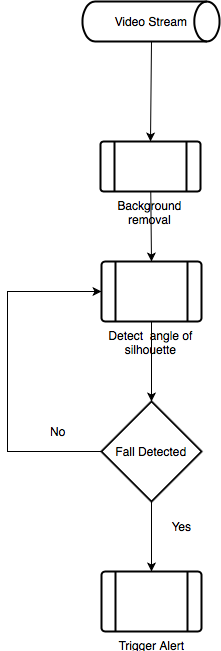
\includegraphics[scale = 0.4]{basicFlowChart.png}
 \caption{Flow Chart showing the five main sections of the Fall-Detection System.}
 \label{fig:basicFlowChart}
\end{figure}

\pagebreak
\noindent
The Flow Chart was used to design the overall architecture of the system. From the chart is was decided that the structure should be to contain four main classes which interact to perform the Fall-Detection and Alert System. The Four main classes were:
\begin{itemize}
\item backgroundRemoval()
	\begin{itemize}
	\item To remove the background from the current frame to leave the silhouette of the user.
	\end{itemize}
\item angleDetection()
	\begin{itemize}
	\item To detect the angle of the silhouette.
	\end{itemize}
\item fallDetection()
	\begin{itemize}
	\item Based on fast change in the angle detect potential falls.
	\end{itemize}
\item fallAlarm()
	\begin{itemize}
	\item Trigger an Alert in the event of a fall.
	\end{itemize}
\end{itemize}

These classes and their interactions are shown in Figure \ref{fig:UMLClassDiagram}.

\begin{figure}[H]
 \centering
 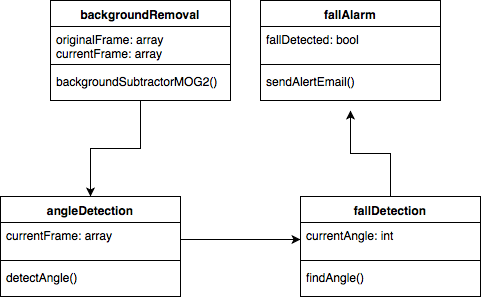
\includegraphics[scale = 0.5]{UMLClassDiagram.png}
 \caption{UML Class Diagram showing the four main classes of the Fall-Detection System.}
 \label{fig:UMLClassDiagram}
\end{figure}

\pagebreak

\section{Development}
The development of the system was done in an iterative manner divided into many sections or iterations. Each print consisted of the development of a small feature or part of the system followed by testing the section which had just been implemented. The tests ensured that the new code added functioned correctly and did not interfere and cause additional bugs in the preexisting code base.

The the order in which the features were implemented in each iteration was based on the importance of the feature and whether it was required before another feature could be added. For example the Silhouette Angle Detection functionality had to be added before the Fall Detection functionality. The five feature each to be added in its own iteration, which collectively make up the development of the Fall-Detection System, were:

\begin{enumerate}
\item Install OpenCV library, Set up Python files and Classes, import and display video feed.
\item Effectively remove the background from the video leaving only the silhouette of the user (if the user is in the frame of the video).
\item Determine the angle of the remaining silhouette.
\item Determine if a fall has occurred.
\item In the event of a fall send an email to the specified recipient.
\end{enumerate}

\subsection{Iteration 1}

The features to be added in the first development iteration of project were relatively simple. This part was the development was just concerned with creating the necessary Python files and installing the OpenCV library which was installed using Homebrew \citep{Homebrew}. The system was created across three different Python ('.py') files to keep the code base tidier and easier to maintain. These were imported using Python's 'import' functionality so that the classes contained in each file could be accessed as if they were all contained within the same file. These imports as well as the required library imports are shown in Listing \ref{PythonImports}. A screen shot showing the files created for the project is shown in Appendix B figure \ref{fig:requiredFiles}. 

\begin{listing}
\begin{minted}{Python}
import cv2, numpy as np
import angleMonitor, fallAction
\end{minted}
\caption{Python code for importing libraries and other '.py' files.}
\label{PythonImports}
\end{listing}
\noindent
The video feed can be displayed using the \textit{videoCapture()} and \textit{imshow()} functions of the OpenCV library. This is shown in Appendix B: Listing \ref{displayInputVideo}.

\subsection{Iteration 2}

The second iteration focused on removing the background from the video stream. This could be done using the functions available in the OpenCV, although there were multiple background subtraction algorithms algorithms available in the library. The available algorithms were:

\begin{itemize}
  \item BackgroundSubtractorMOG
  \item BackgroundSubtractorMOG2
  \item BackgroundSubtractorGMG
\end{itemize}
\noindent
The algorithm which was used was \textit{BackgroundSubtractorMOG2} as this performed the best background subtraction and also had acceptable performance, removing the background from each frame without too much delay. This algorithm was also combined with the Morphological Operations Dilate and Erode, as well as binary thresholding to remove any noise which was left behind after the \textit{backgroundSubtractionMOG2} algorithm. The end result of the background subtraction in conjunction with the Morphological Operations is shown in Appendix B: Figure \ref{fig:backgroundSub} and a snippet of the Python code behind this is shown in Appendix B: Listing \ref{bgSubPython}.

\subsection{Iteration 3}

This development iteration focused on determining the angle of the remaining silhouette in the image. This was done using three of the available functions of OpenCV. Firstly, it needed to be determined whether the remaining non-zero pixels in the image array constituted a silhouette being present. This was done by measuring the area of the the single area. The required area range which a human would occupy was found using trial and error. If an object is present in the frame inside this area range it is assumed to be a human figure. An ellipse is placed around this figure using OpenCV's \textit{fitEllipse()} function and is displayed on the video output for testing. A line is then placed through the Ellipse along its major axis. The angle of this line will then be equal to the angle at which the person is positioned in the frame. The result of this angle detection is shown in Appendix B: Figure \ref{fig:angleDetectionExample} and a code snippet of the \textit{angleDetection()} function is in Appendix B: Listing \ref{angleDetectionPython}.

\pagebreak
\section{Testing}
The testing of the Fall-Detection System used a mixture of White-box and Black-box testing. This was to ensure that the system was not only functioning to complete to complete the general task correctly but was also working efficiently. Each section of the system was tested interdependently following its implementation. Black-box testing was the primary testing method as the much of the system was built upon functions built into the OpenCV library making White-box testing difficult and perhaps unnecessary.

The background subtraction was the first part of the system to be tested (it was also the first to be implemented). This was done as White-box test by watching the video output after it had been processed by the \textit{backgroundSubtraction()} function to see how effectively it was removing the background and minimising noise. An example of the output of the first iteration of the background removal is shown in Appendix C: Figure \ref{fig:bgSubNoise}. After and testing and making improvements by trial-and-error the final background removal function was able to remove the background pixels of the video whilst leaving effectively removing noise. This is shown in Appendix C: Figure \ref{fig:fallDetected}.

Once the Angle-Detection system had been implemented it was also tested. This was done in a similar manner to the testing of the background subtraction. The output of the angle detection function was displayed both on the on-screen silhouette as well as in some text at the top of the output image to make this part of the system easier to debug (shown in Appendix C: Figure \ref{fig:fallDetected}). The angle of the on-screen line was measured to make certain that the measured angle matched the one being detected by the system.

The final part of the Fall-Detection system to be implemented and tested was the fall detection system. This part could be tested using both White and Black-box testing methods. As the alerts system had not yet been created, when a fall was detected the program would output the string "Fall Detected" to the terminal. This allowed the testing of this functionality without having to implement the full alert system (this output after a detected fall is shown in Appendix C: Figure \ref{fig:fallDetectedOutput}. When ever the silhouette fell the the test video the output in the terminal read "Fall Detected", showing that it was functioning correctly.

\section{Operations and Maintenance}

The Fall-Detection system requires little maintenance once installed. This is because the system is designed to run without any direct interaction from the user (this was discussed previously in section 1.4) The only maintenance that could potentially be required would be to reboot the system in the event that it is not processing the live video feed in real-time and has run out of available memory storing this backlog of video frames.

\chapter{Project Conclusion}

\chapter{Reflective Analysis}

%time, methodology, learning, research, problems installing the library

%References
\renewcommand\bibname{References}
\addcontentsline{toc}{chapter}{References}
\bibliography{references.bib}
\pagebreak
\clearpage

%Appendices
\appendix
\section{Appendices}
\subsection{Appendix A}

\begin{figure}[h]
 \centering
 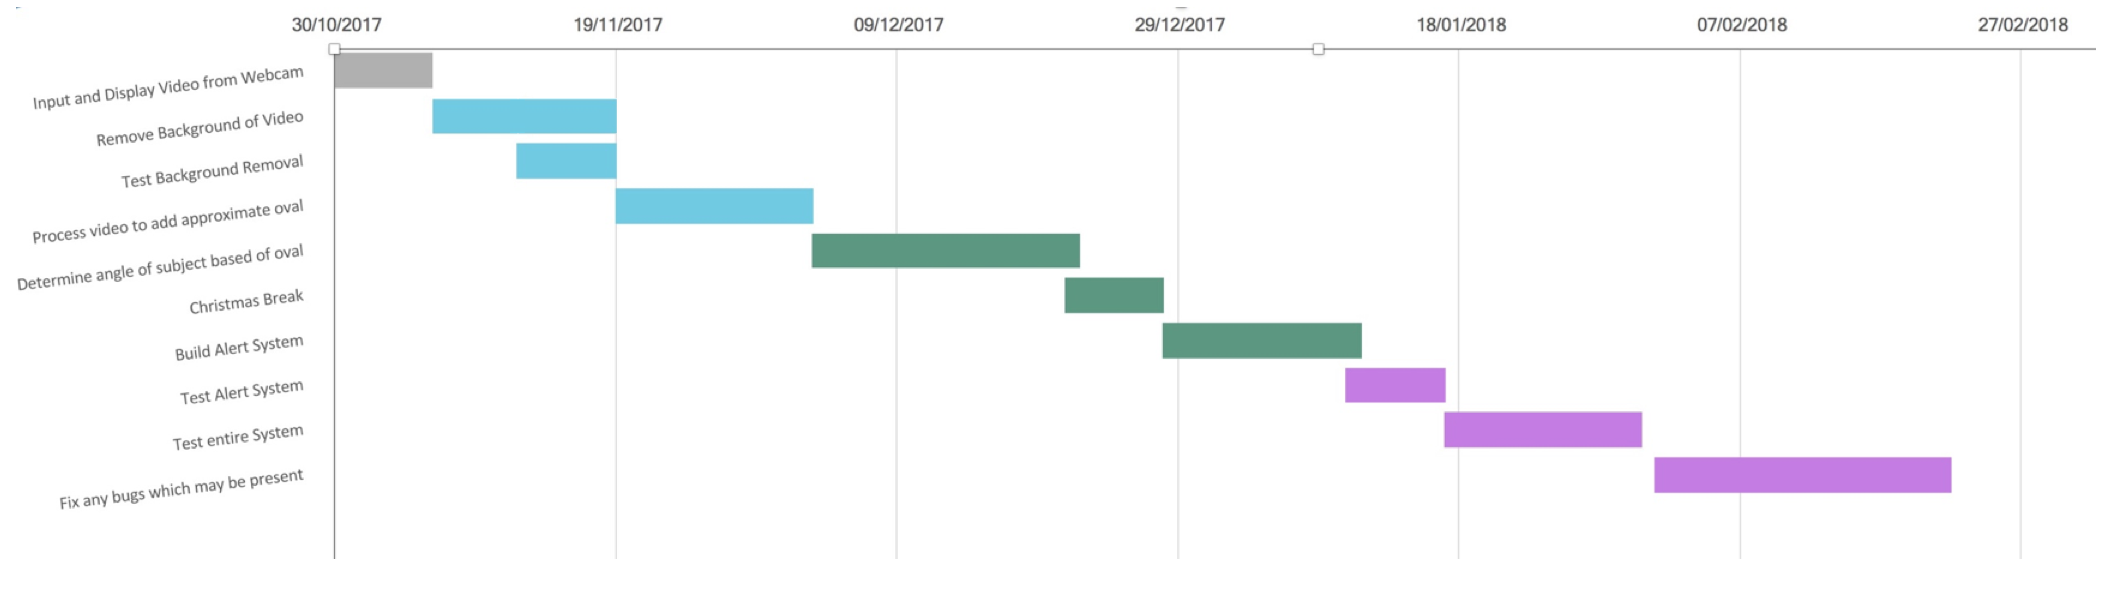
\includegraphics[scale = 0.33]{Original_gantt_chart.png}
 \caption{Original Gantt Chart for the planned project timescale.}
 \label{fig:OriginalGantt}
\end{figure}

\begin{figure}[h]
 \centering
 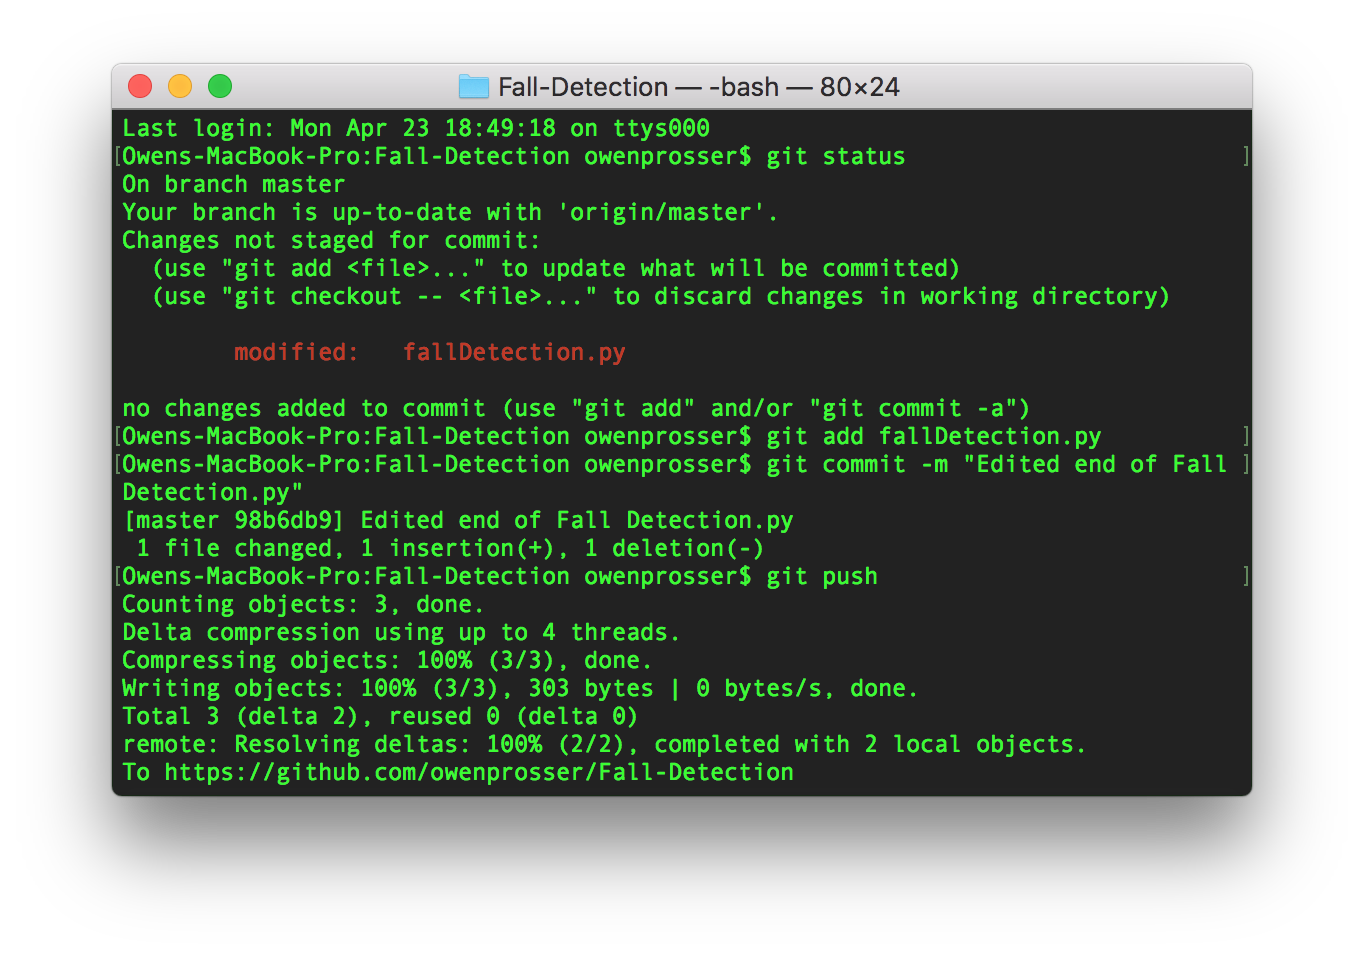
\includegraphics[scale = 0.55]{gitpush.png}
 \caption{Example of git commit and push commands.}
 \label{fig:GitCommitPush}
\end{figure}

\begin{figure}[H]
 \centering
 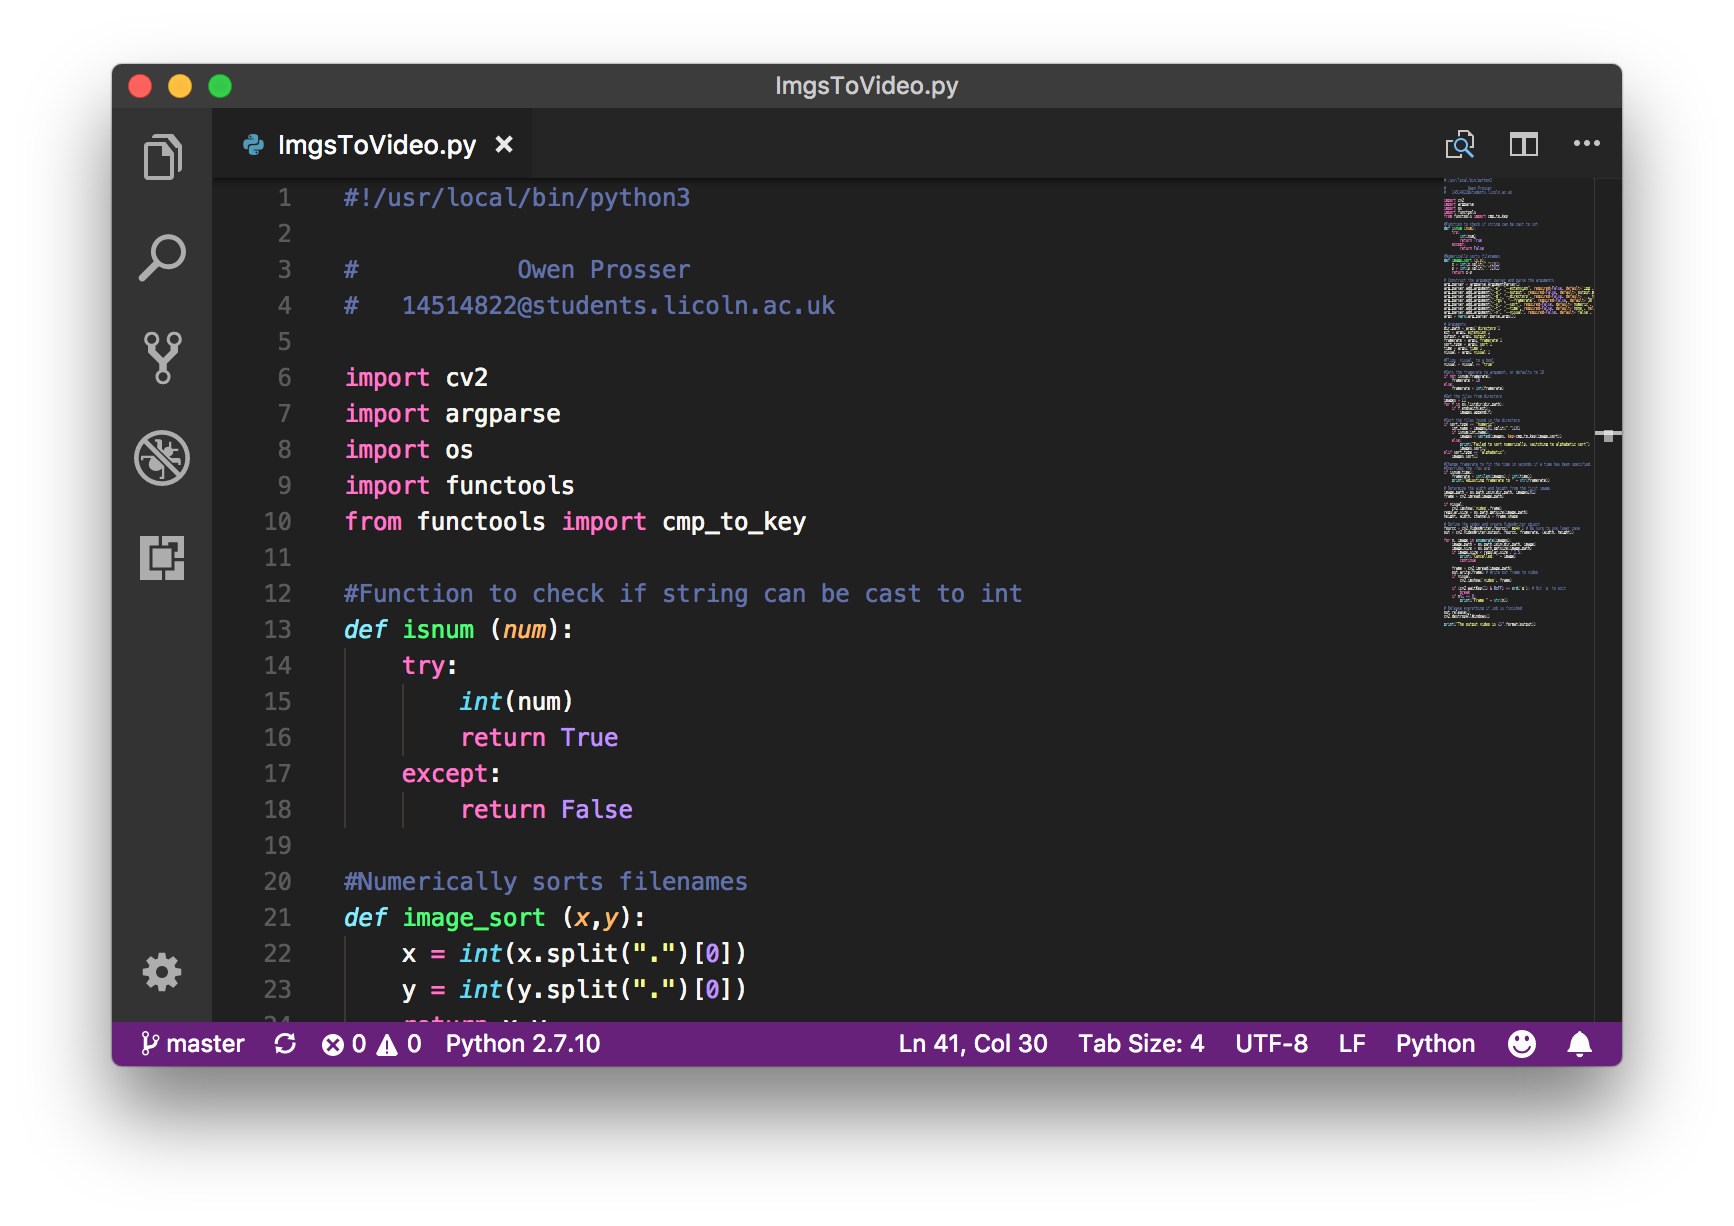
\includegraphics[scale = 0.4]{VSCode.png}
 \caption{Example of Python code in Visual Studio Code with Syntax Highlighting}
 \label{fig:VSCode}
\end{figure}

\begin{figure}[H]
 \centering
 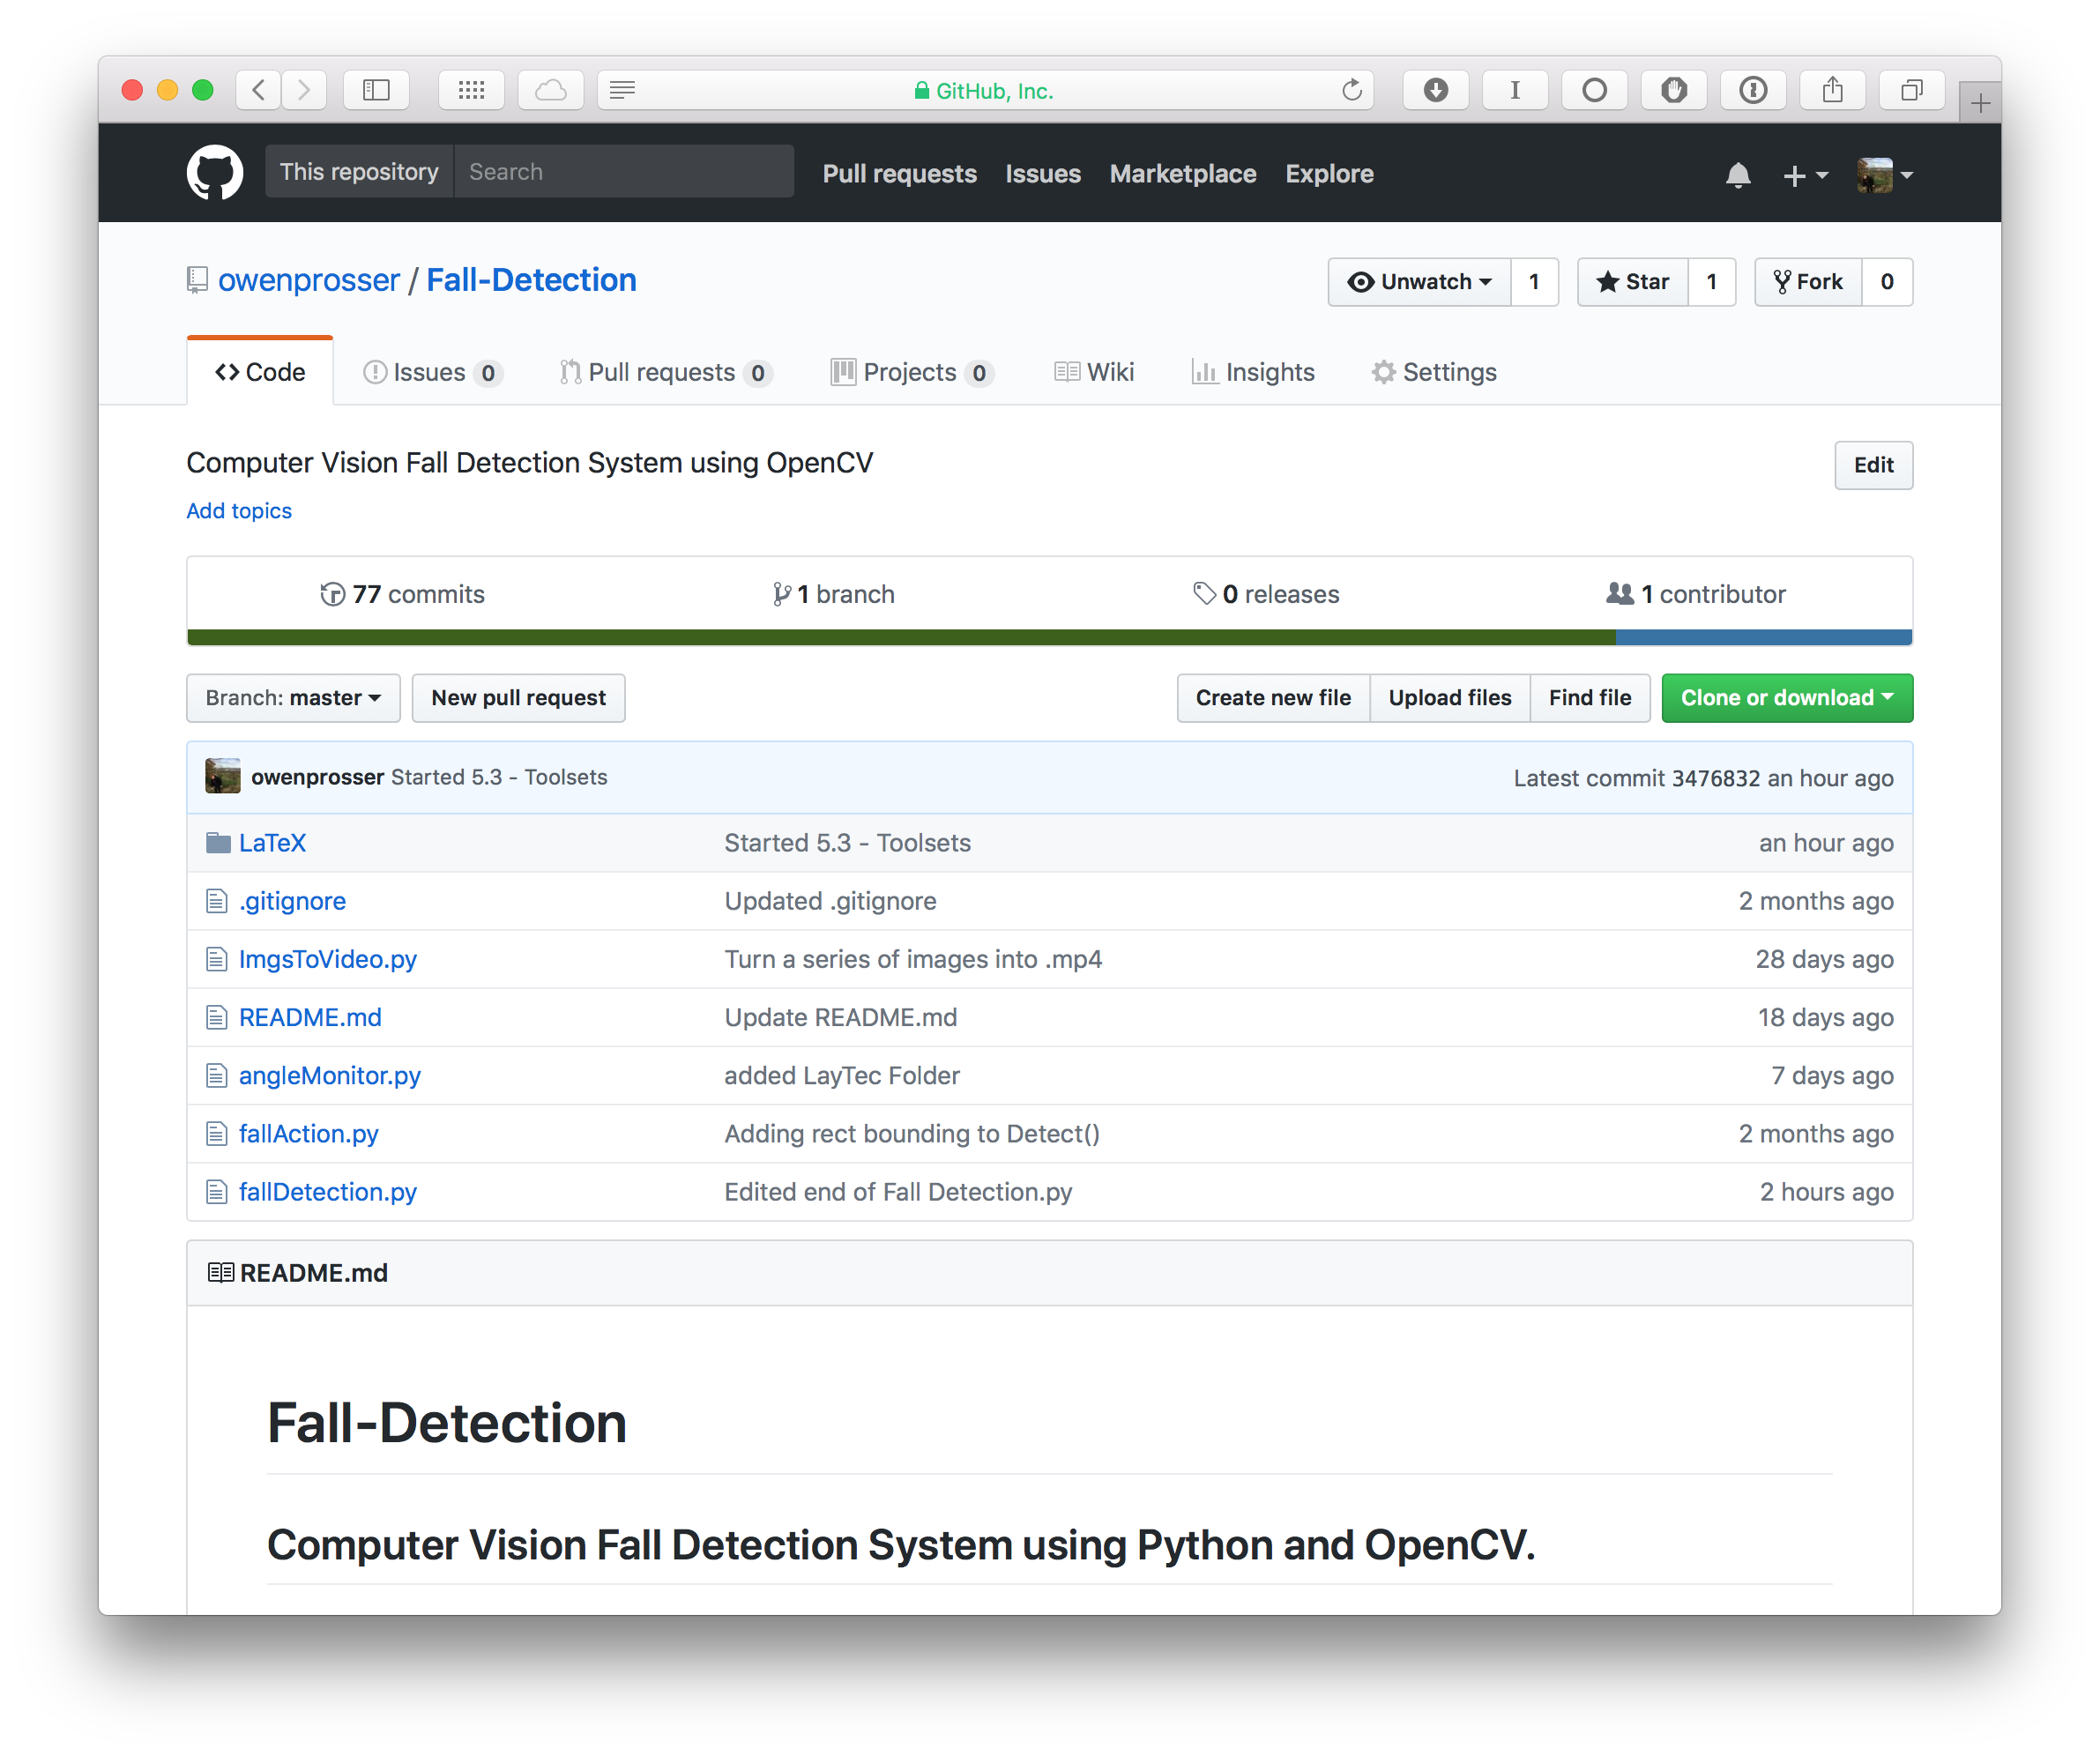
\includegraphics[scale = 0.14]{GitRepo.png}
 \caption{Screen shot of the Git Repository Hosted on http://github.com.}
 \label{fig:GitRepo}
\end{figure}

\subsection{Appendix B}

\begin{figure}[H]
 \centering
 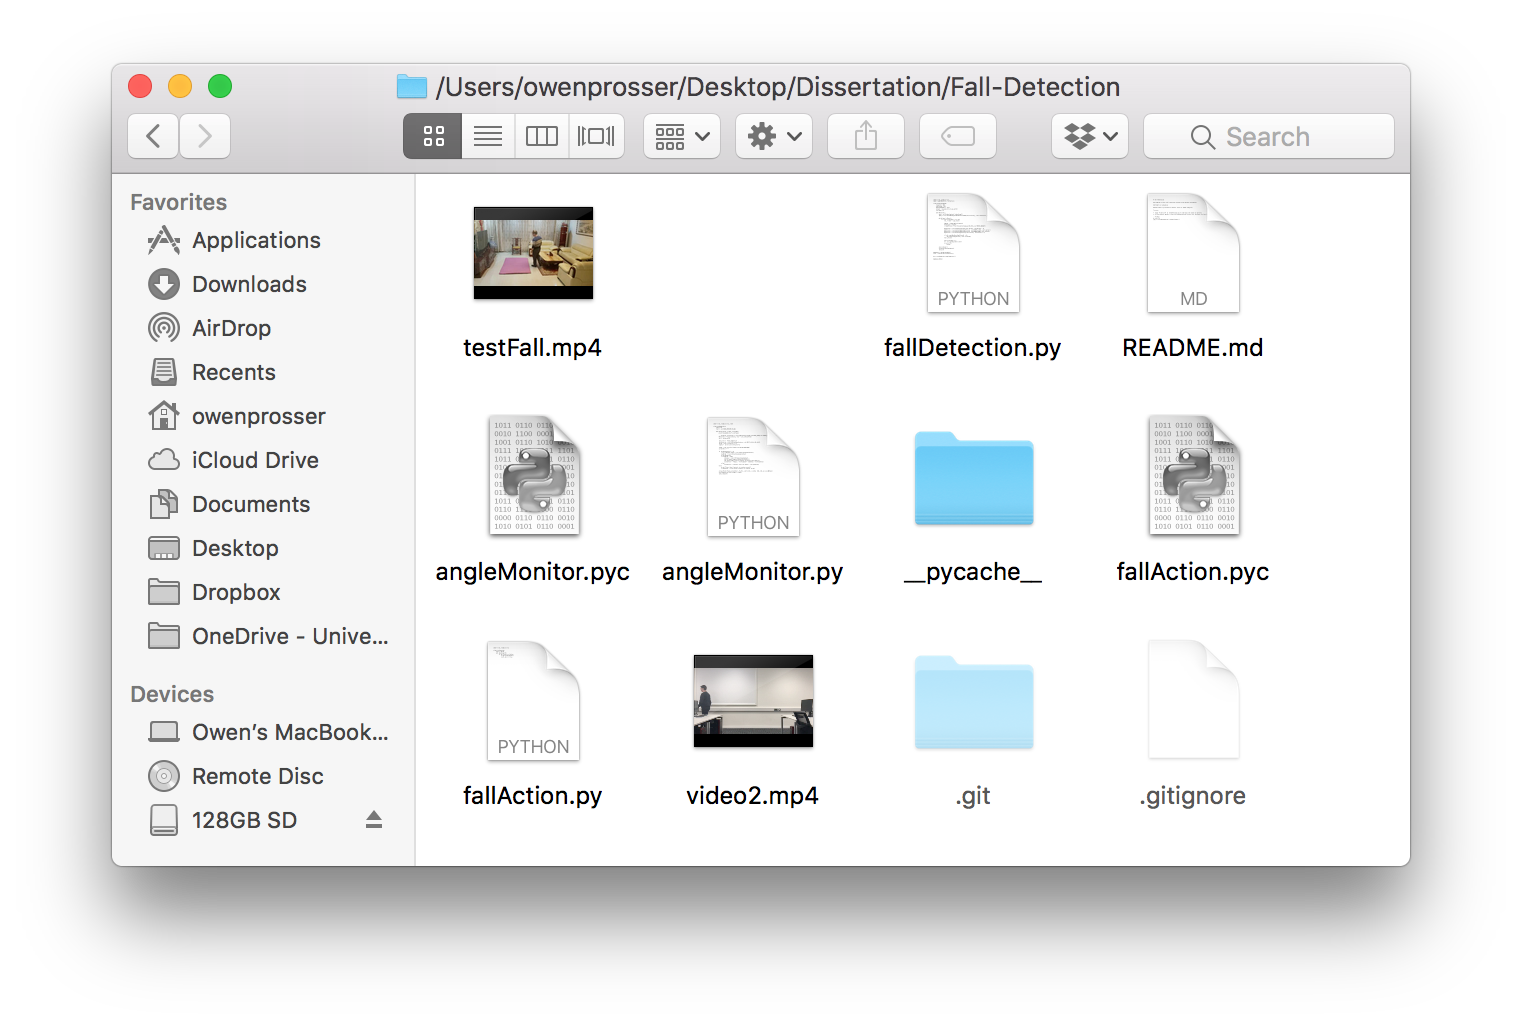
\includegraphics[scale = 0.5]{requiredFiles.png}
 \caption{'.py' and other files needed for the system.}
 \label{fig:requiredFiles}
\end{figure}

\begin{listing}
\begin{minted}{Python}
while(cap != None):
  cap = cv2.VideoCapture(0)
  if (self.curFrame % 1 == 0):
    ret, frame = cap.read()
    cv2.imshow("Current Frame", frame)
    self.curFrame += 1
    k = cv2.waitKey(30) & 0xff
  if k == 27:
  	break
cap.release()
cv2.destroyAllWindows()
return 0
\end{minted}
\caption{Python code snippet to show live webcam feed using OpenCV.}
\label{displayInputVideo}
\end{listing}

\begin{figure}[H]
 \centering
 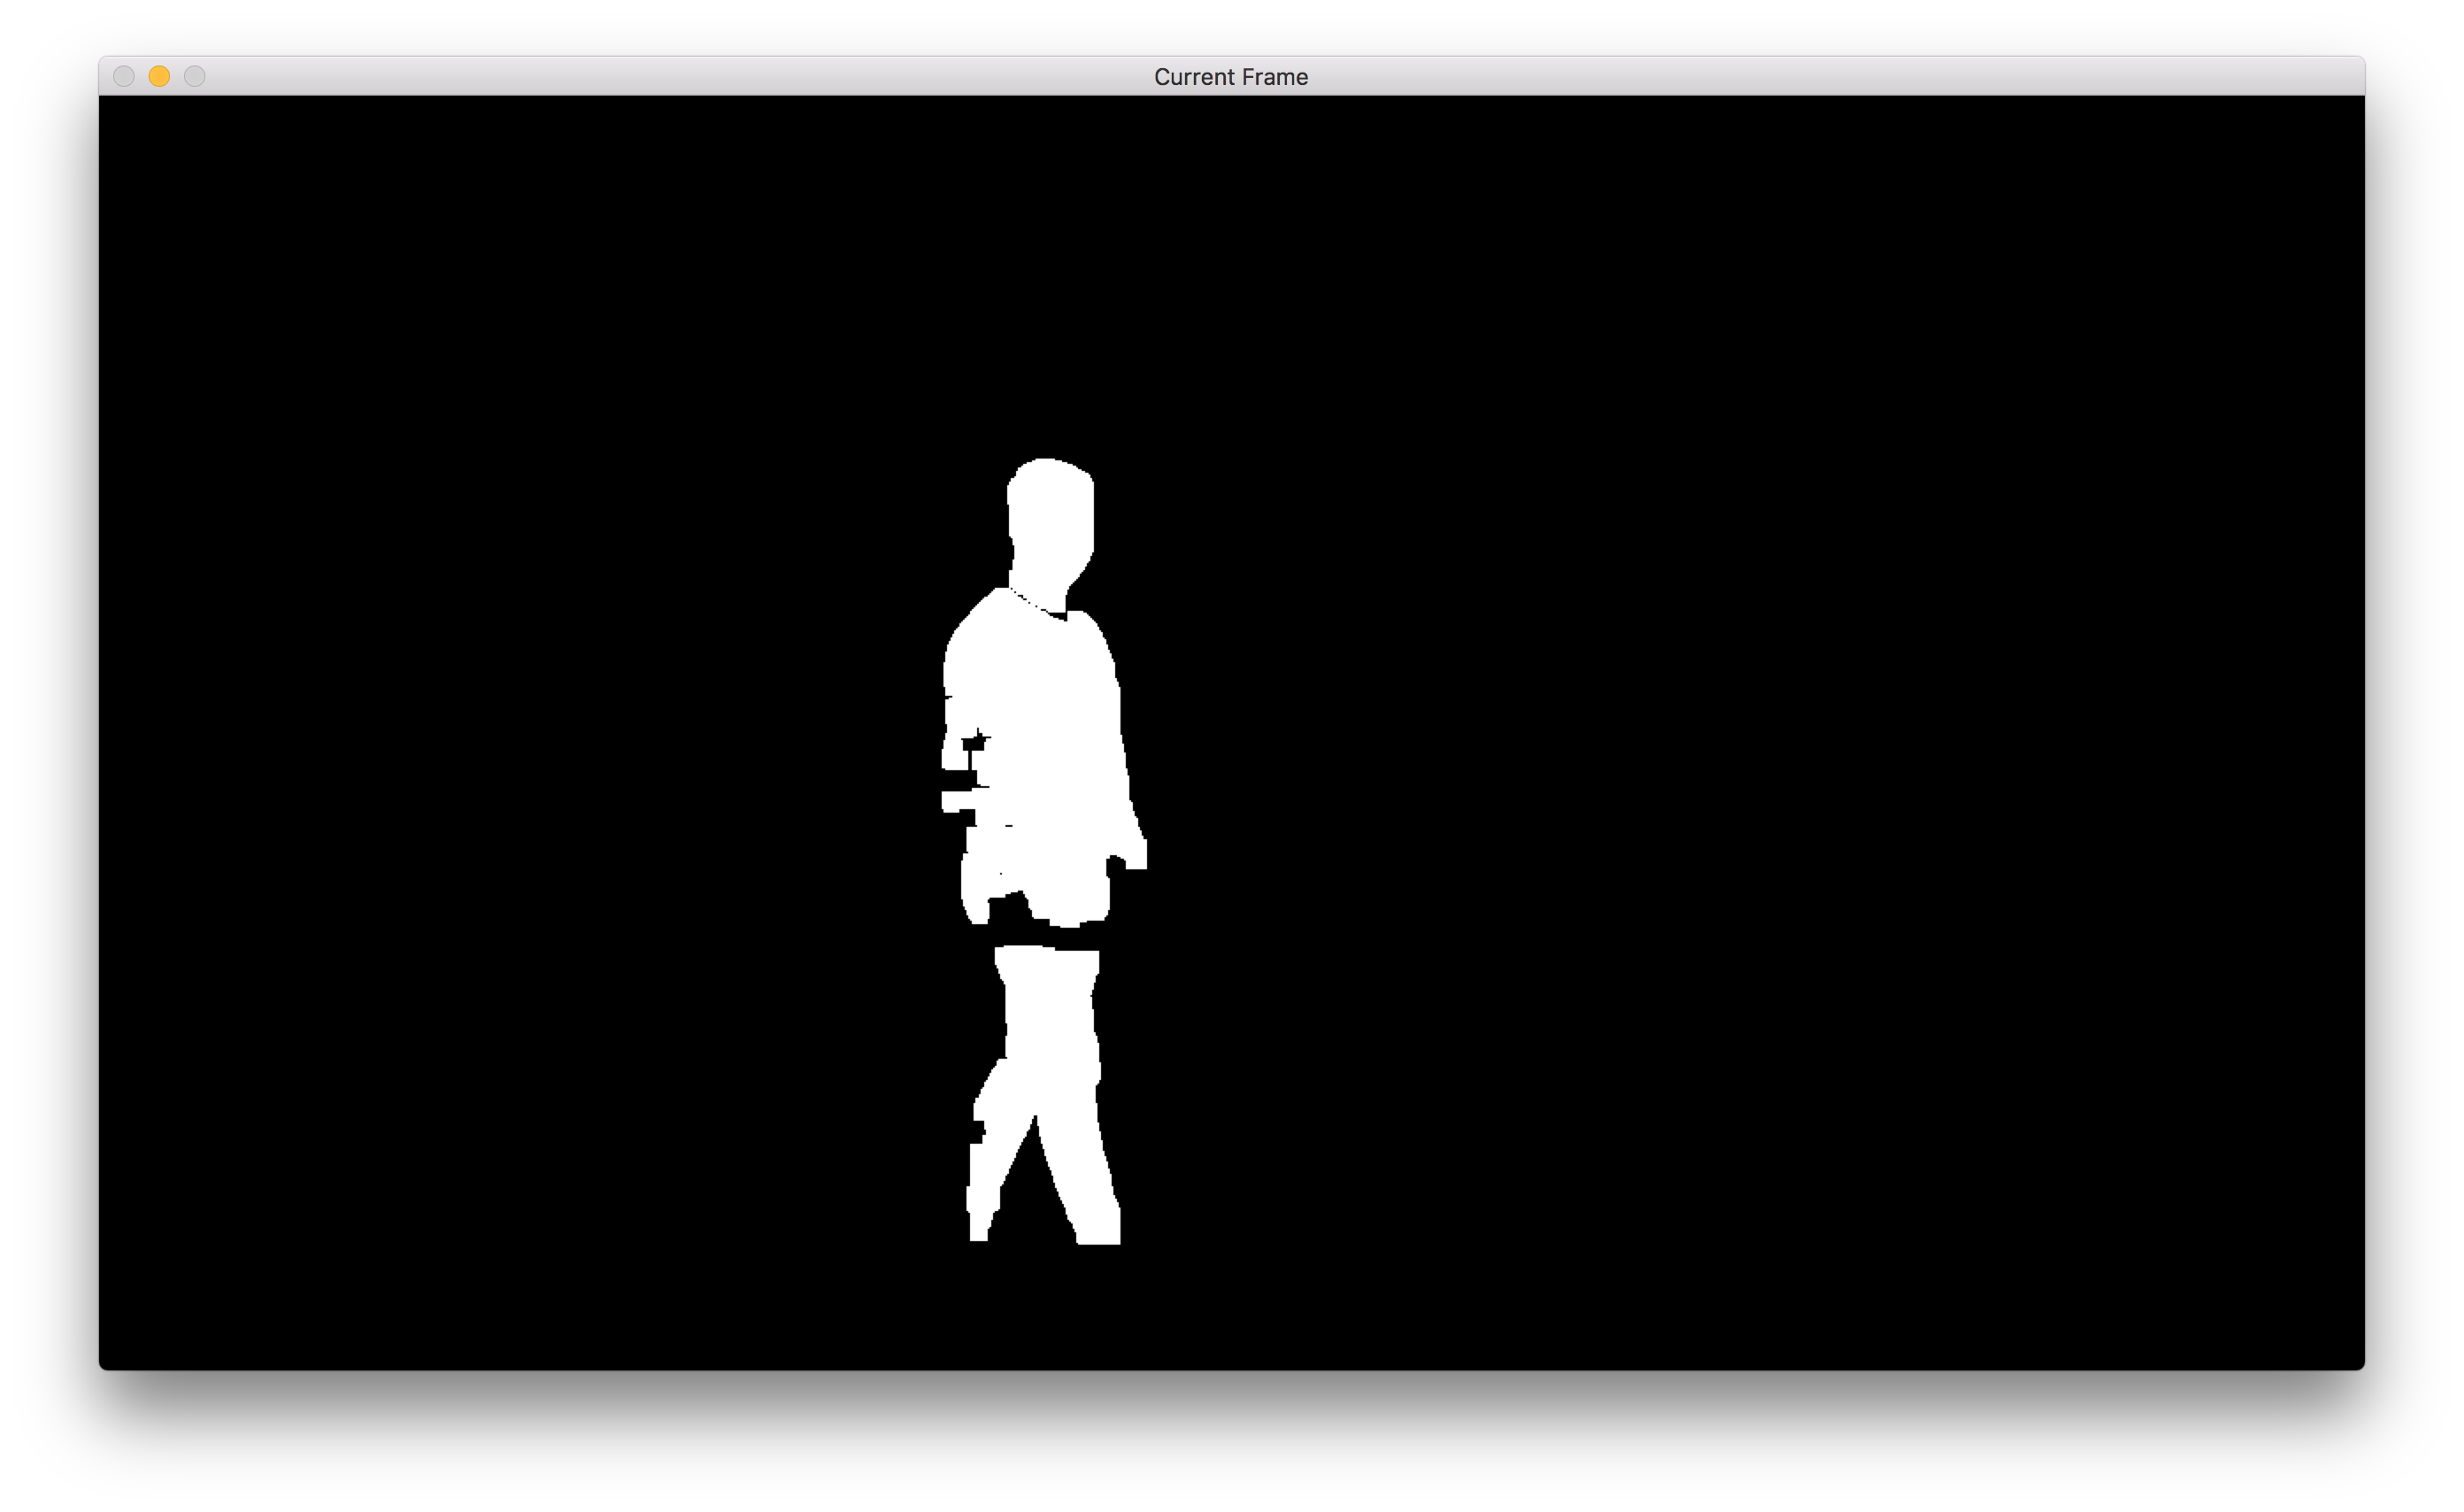
\includegraphics[scale = 0.22]{bgSubExample.png}
 \caption{Screen shot showing the effectiveness of the backgroudSubtractorMOG2() algorithm with Morphological Operations.}
 \label{fig:backgroundSub}
\end{figure}

\begin{listing}
\begin{minted}{Python}
def MOG(self):
  cap = cv2.VideoCapture('video2.mp4')
  fgbg = cv2.createBackgroundSubtractorMOG2(self.history, 
  self.varThresh ,self.detectShadows)
  while(cap != None):
    if (self.curFrame % 1 == 0):
      ret, frame = cap.read()
      fgmask = fgbg.apply(frame,0)
      bgrThresh = fgmask
      _, bgrThresh = cv2.threshold(fgmask,250,255,cv2.THRESH_BINARY)
      bgrThresh = cv2.erode(bgrThresh,self.kernel, iterations = 1)
      bgrThresh = cv2.morphologyEx(bgrThresh, cv2.MORPH_CLOSE, self.kernel)
      bgrThresh = cv2.morphologyEx(bgrThresh, cv2.MORPH_OPEN, self.kernel)
      bgrThresh = cv2.dilate(bgrThresh,self.kernel, iterations = 1)
      if cv2.countNonZero(bgrThresh) > 0:
      	det.Detect(bgrThresh, self.curFrame)
      self.curFrame += 1
      k = cv2.waitKey(30) & 0xff
      if k == 27:
      	break
cap.release()
cv2.destroyAllWindows()
return 0
\end{minted}
\caption{Python for Background Subtraction and Morphological Operations.}
\label{bgSubPython}
\end{listing}

\begin{figure}[H]
 \centering
 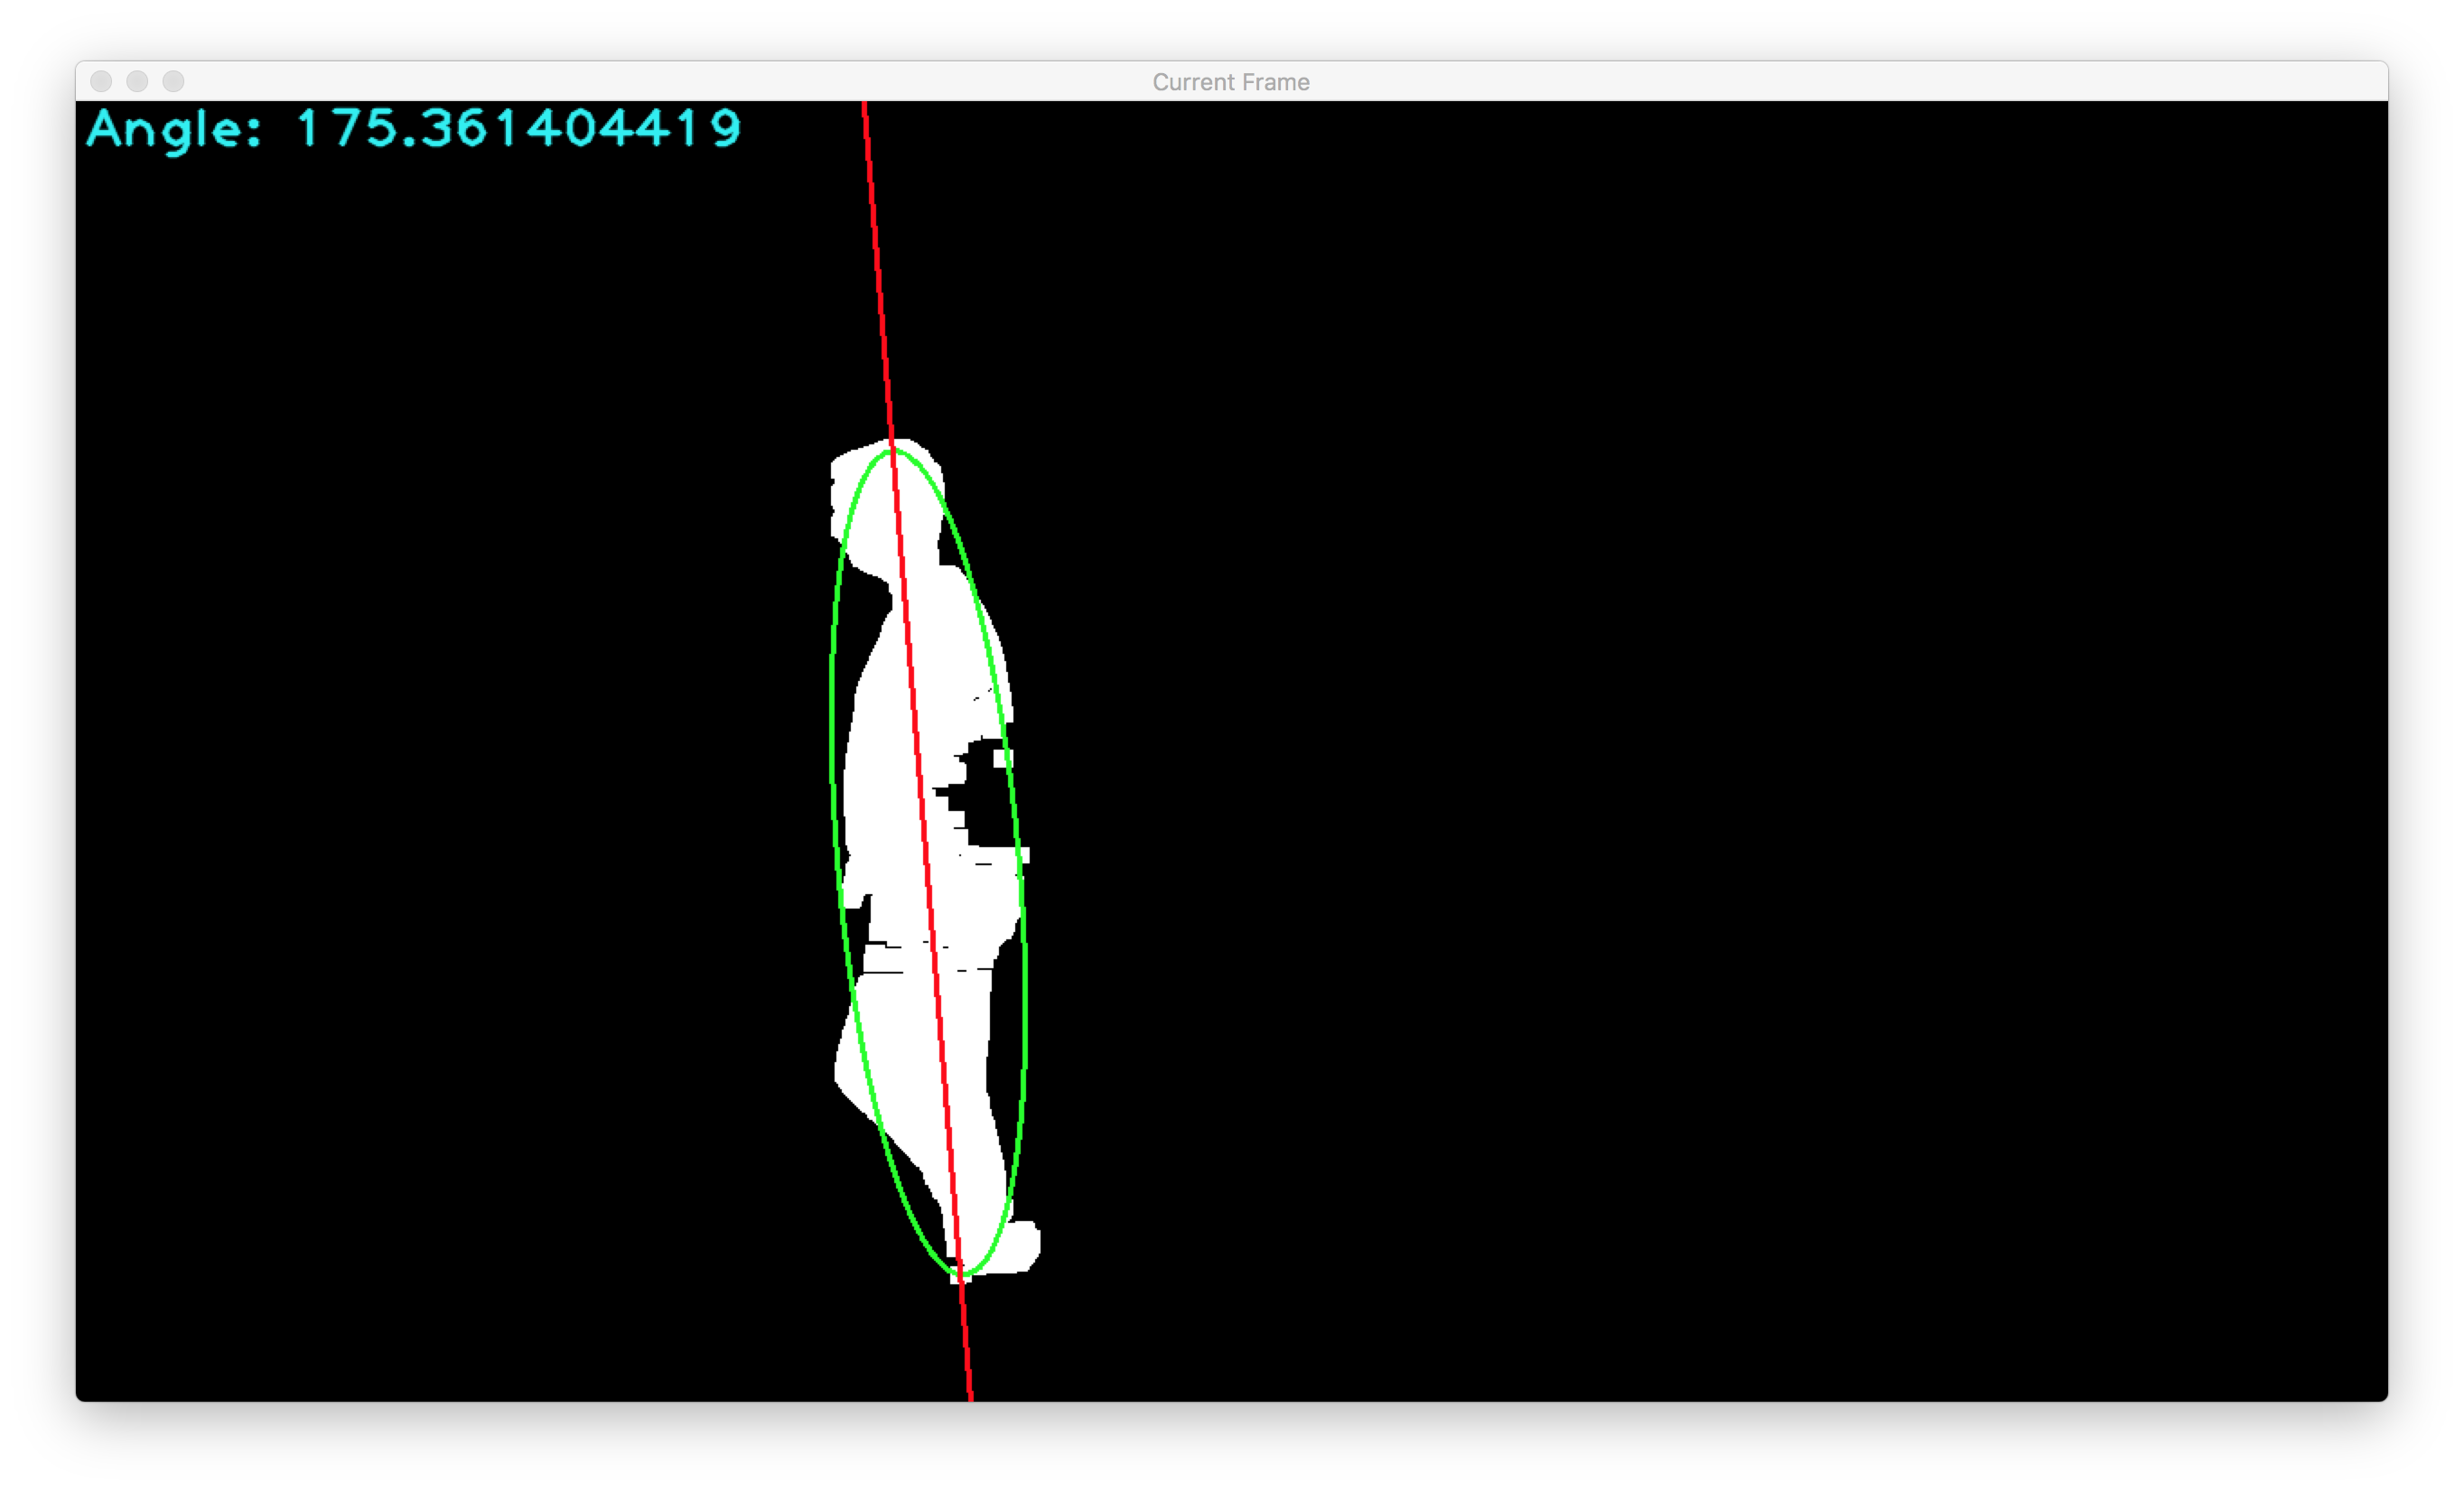
\includegraphics[scale = 0.22]{angleExample.png}
 \caption{Screen shot showing the output from the \textit{angleDetection()} function.}
 \label{fig:angleDetectionExample}
\end{figure}

\begin{listing}
\begin{minted}{Python}
def Detect(self, frame, curFrame):
  _, contours, hierarchy = cv2.findContours(frame,cv2.RETR_TREE,
  cv2.CHAIN_APPROX_SIMPLE)
  maxContour = max(contours, key = cv2.contourArea)
  cnt = contours[0]

  rows,cols = frame.shape[:2]
  [vx,vy,x,y] = cv2.fitLine(maxContour, cv2.DIST_L2,0,0.01,0.01)
  lefty = int((-x*vy/vx) + y)
  righty = int(((cols-x)*vy/vx)+y)

  frame = cv2.cvtColor(frame,cv2.COLOR_GRAY2RGB)
  screenText = ""

  if len(maxContour) > 4:
    (x,y),(MA,ma),angle = cv2.fitEllipse(maxContour)
    maxArea = cv2.contourArea(maxContour)
    print(maxArea)
    if maxArea > 100:
      ellipse = cv2.fitEllipse(maxContour)
      cv2.ellipse(frame,ellipse,(0,255,0),2)
      cv2.line(frame,(cols-1,righty),(0,lefty),(0,0,255),2)
      screenText = 'Angle: '+str(angle)
\end{minted}
\caption{Python code for angle detection.}
\label{angleDetectionPython}
\end{listing}

\subsection{Appendix C}

\begin{figure}[H]
 \centering
 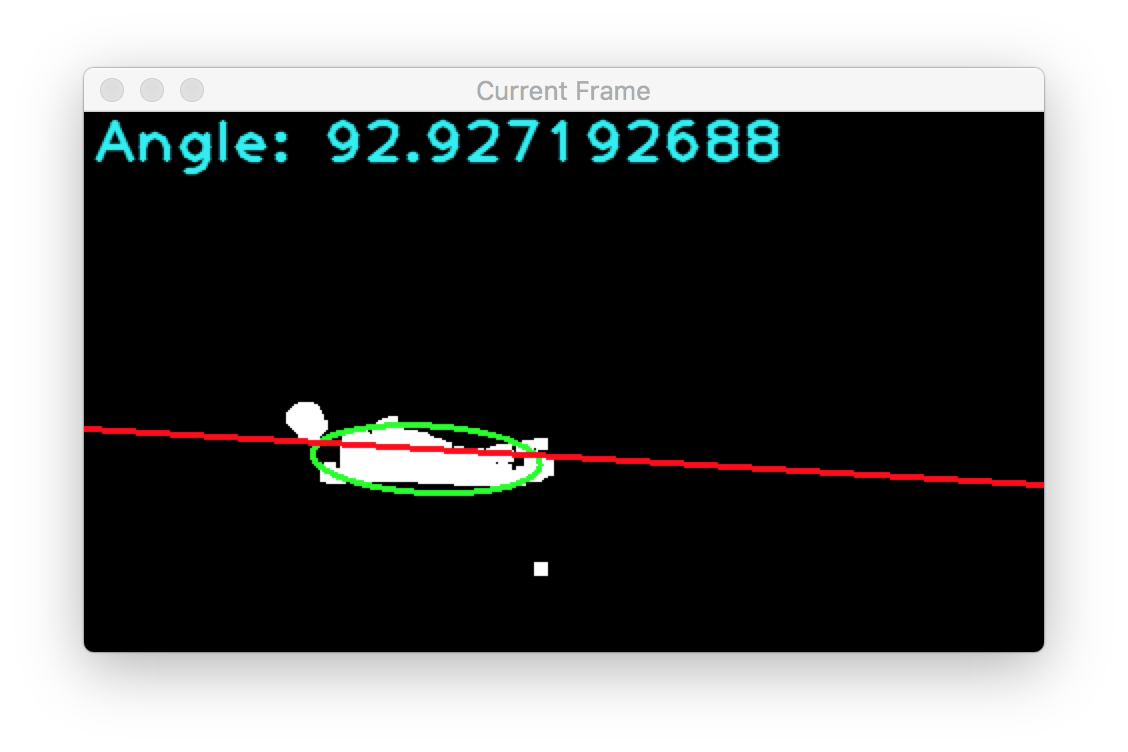
\includegraphics[scale = 0.6]{fallDetected.png}
 \caption{Screen shot showing the output during the detection of a fall.}
 \label{fig:fallDetected}
\end{figure}

\begin{figure}[H]
 \centering
 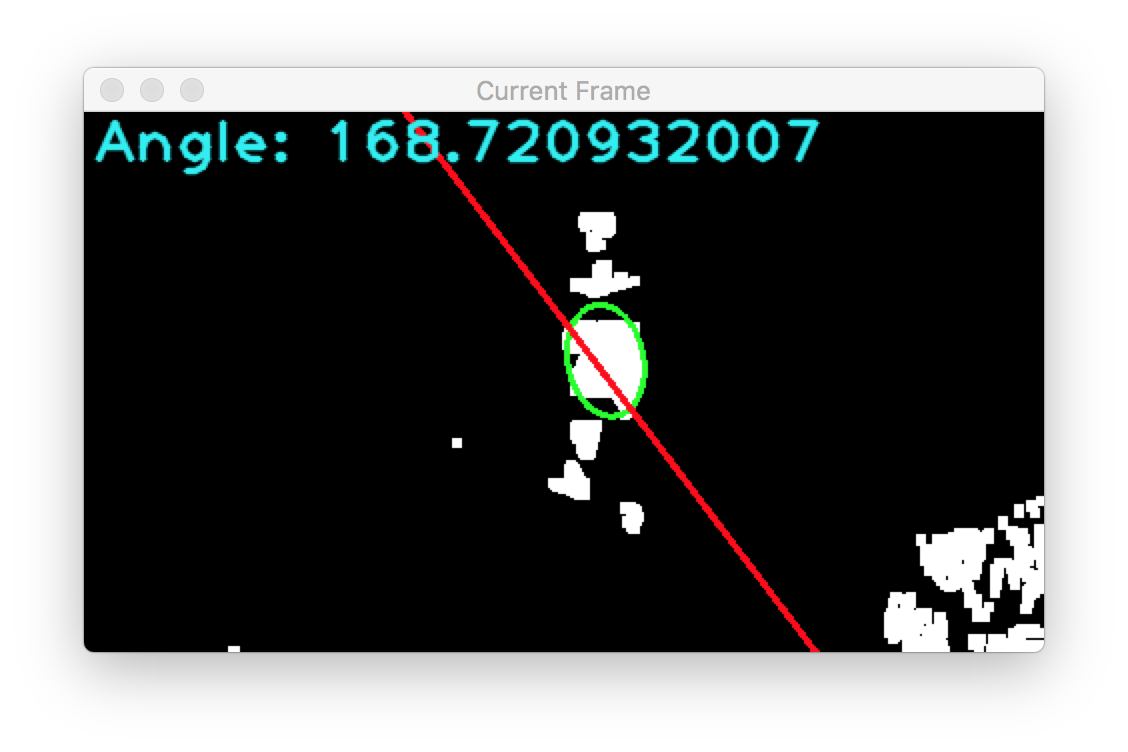
\includegraphics[scale = 0.6]{bgSubNoise.png}
 \caption{Screen shot showing the remaining noise after processing by an early version of the background subtraction function.}
 \label{fig:bgSubNoise}
\end{figure}

\begin{figure}[H]
 \centering
 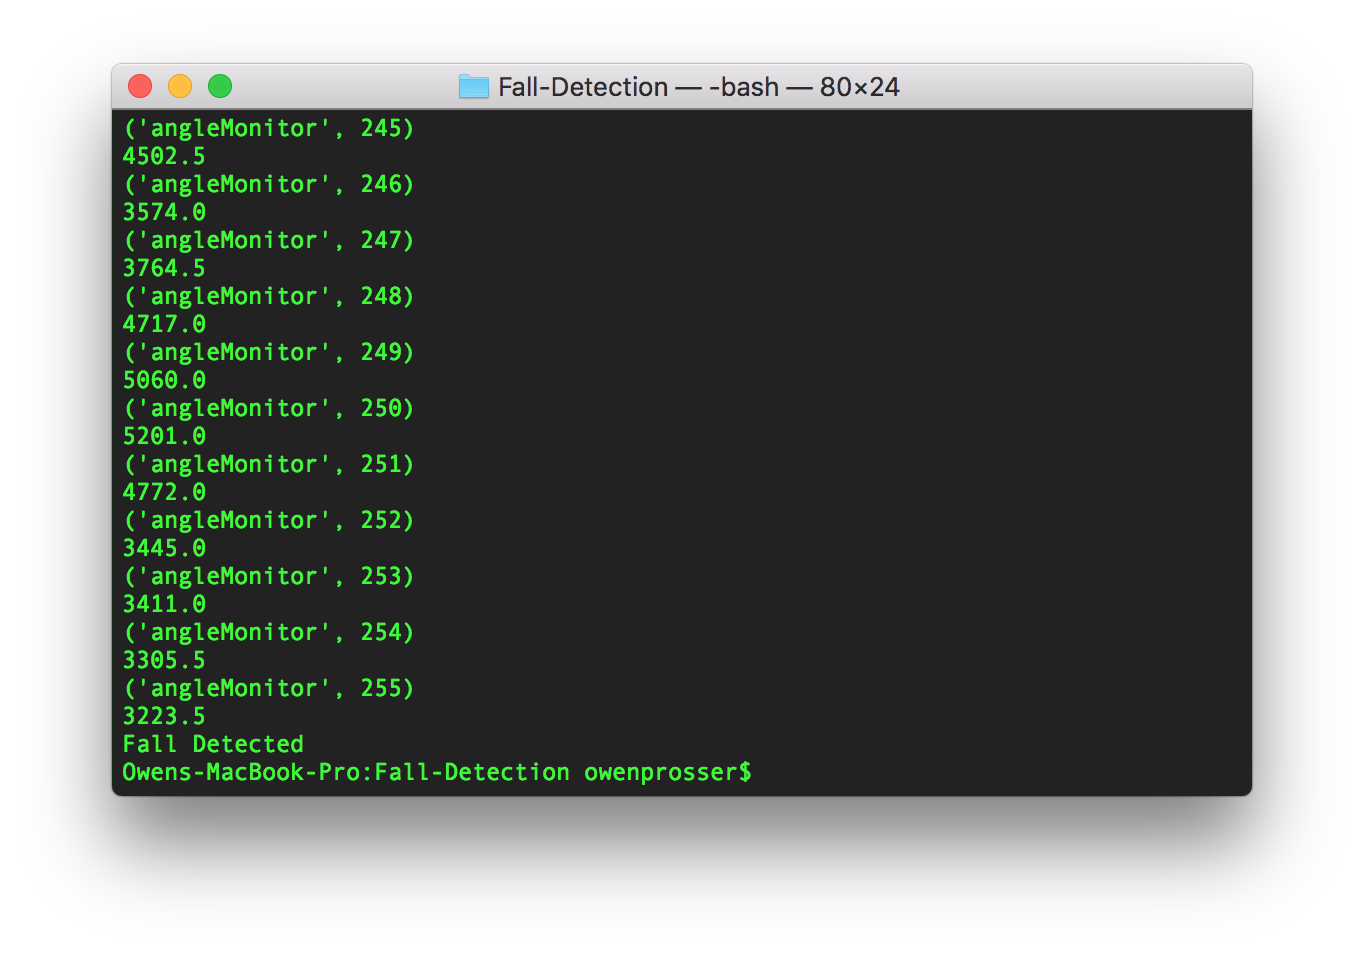
\includegraphics[scale = 0.5]{fallDetectedOutput.png}
 \caption{Screen shot showing the output to the terminal in the event of detecting a fall.}
 \label{fig:fallDetectedOutput}
\end{figure}

\end{document}